%!TEX root = ../main.tex
\section{Simulations}
Before the controllers can be tested on the real system a simulation must be done. The controllers that have been chosen are the IPD and PI, where PI is the PID controller with $K_D$ set to 0. Speed control is simulated at two different angular velocities, \todo{To different step signals ? - Mikkel}200~rad/s and~125 rad/s. To prevent the saturation limit to be reached, the settling time is set to 0.1~ms.\todo{why settling time 0.1 and not 0.01}
\todo[inline]{Why are these choosen? -Mikkel}
\begin{figure}[h!]
	\centering
	\begin{subfigure}[b]{0.45\textwidth}
		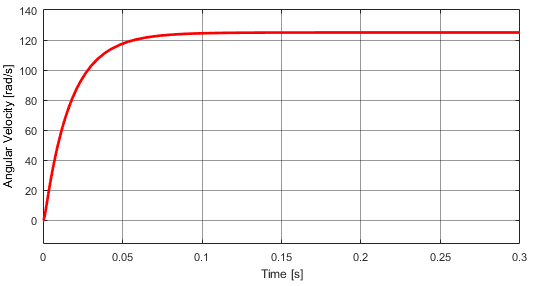
\includegraphics[width=\textwidth]{graphics/PI_single125}
		\caption{PI Speed control at 125 rad/s.}
		\label{fig:pisingle125}
	\end{subfigure}
	~ %add desired spacing between images, e. g. ~, \quad, \qquad, \hfill etc. 
	%(or a blank line to force the subfigure onto a new line)
	\begin{subfigure}[b]{0.45\textwidth}
		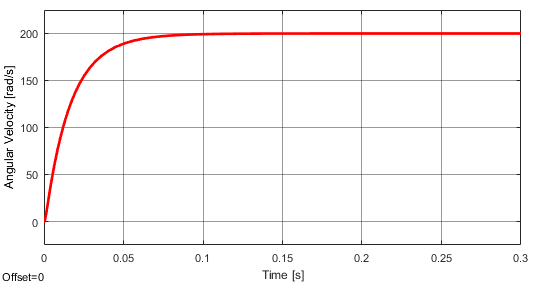
\includegraphics[width=\textwidth]{graphics/PI_single200}
		\caption{PI Speed control at 200 rad/s.}
		\label{fig:pisingle200}
	\end{subfigure}
	\caption{The PI controller at two different angular velocities. It is noticed that the desired settling time is reached in both cases.}\label{fig:pisingle}
\end{figure}






\begin{figure}[h!]
	\centering
	\begin{subfigure}[b]{0.45\textwidth}
		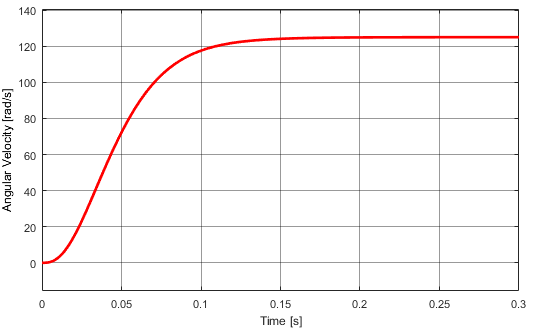
\includegraphics[width=\textwidth]{graphics/IPD_single125}
		\caption{IPD Speed control at 125 rad/s.}
		\label{fig:ipdsingle125}
	\end{subfigure}
	~ %add desired spacing between images, e. g. ~, \quad, \qquad, \hfill etc. 
	%(or a blank line to force the subfigure onto a new line)
	\begin{subfigure}[b]{0.45\textwidth}
		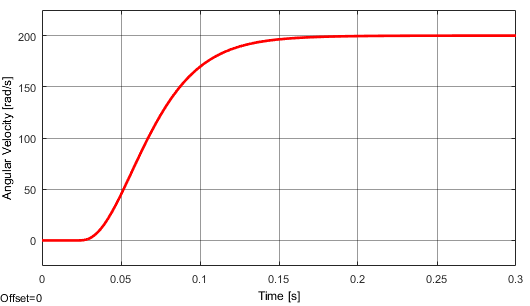
\includegraphics[width=\textwidth]{graphics/IPD_single200}
		\caption{IPD Speed control at 200 rad/s.}
		\label{fig:ipdsingle200}
	\end{subfigure}
	\caption{The IPD controller at two different angular velocities. A delay is introduced. The desired settling time is reached from when the controller responses.}\label{fig:ipdsingle}
\end{figure}
\todo{The sentence may need to be expressed again? "The desired...the controller}

\todo[inline][We should be able to find out where the delay comes from? - Mikkel]
The simulation confirms that the controllers behave similar for both simulated angular velocities as seen in figures~\ref{fig:pisingle} and~\ref{fig:ipdsingle}. Both the PI and IPD achieve to settle within the specified settling time. However, an unexplained delay is introduced in the beginning of the IPD controller response. That delay does not affect the system response in other way than offsetting it.

\begin{figure}[h!]
	\centering
	\begin{subfigure}[b]{0.45\textwidth}
		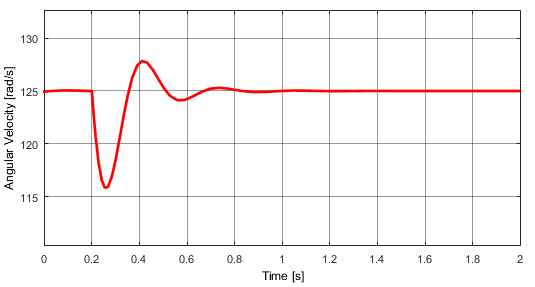
\includegraphics[width=\textwidth]{graphics/PI_load125}
		\caption{PI Speed control at 125 rad/s.}
		\label{fig:piload125}
	\end{subfigure}
	~ %add desired spacing between images, e. g. ~, \quad, \qquad, \hfill etc. 
	%(or a blank line to force the subfigure onto a new line)
	\begin{subfigure}[b]{0.45\textwidth}
		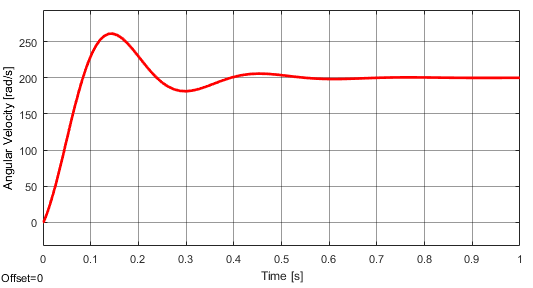
\includegraphics[width=\textwidth]{graphics/PI_load200}
		\caption{PI Speed control at 200 rad/s.}
		\label{fig:piload200}
	\end{subfigure}
	\caption{The PI controller at two different angular velocities with added load. Desired settling time is not reached. Instead, it introduces an overshoot and does not become stable until it is close to 1s.}
	\label{fig:piload}
\end{figure}

\begin{figure}[h!]
	\centering
	\begin{subfigure}[b]{0.45\textwidth}
		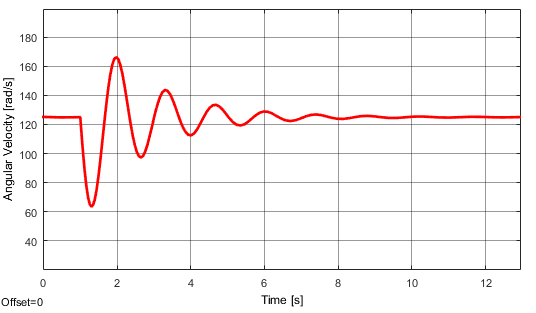
\includegraphics[width=\textwidth]{graphics/IPD_load125}
		\caption{IPD Speed control at 125 rad/s.}
		\label{fig:ipdload125}
	\end{subfigure}
	~ %add desired spacing between images, e. g. ~, \quad, \qquad, \hfill etc. 
	%(or a blank line to force the subfigure onto a new line)
	\begin{subfigure}[b]{0.45\textwidth}
		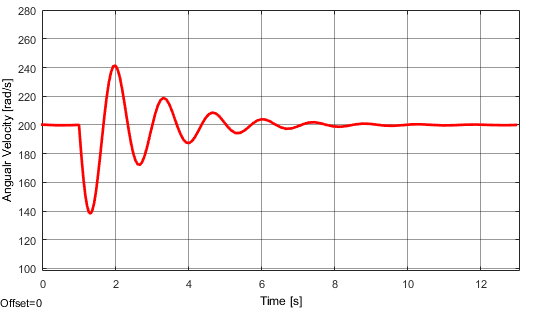
\includegraphics[width=\textwidth]{graphics/IPD_load200}
		\caption{IPD Speed control at 200 rad/s.}
		\label{fig:ipdload200}
	\end{subfigure}
	\caption{The IPD controller at two different angular velocities with added load. The desired settling time is far from being reached. The system becomes stable at around 13s.}
	\label{fig:ipdload}
\end{figure}
\todo{5.4 figures is referring to IPD controller, right? PI was written here.}

When the system has reached the stable output a load step is introduced.
When the load step is added, the IPD controller seems to have a hard time to settle, as it can be shown from figure~\ref{fig:ipdload}. The systems does not reach the stable condition until after 13s. This result could have been estimated thus the controllers were designed with only a single motor in mind. Added load changes the system behaviour and should be controlled with different controller gains.\todo{Catalin: I don't understand the sentence "This result...mind"}
